\section{Verifying Eio's Broadcast}
\label{sec:broadcast}

% <!-- In general, what is Broadcast/CQS? -->

In this section we go into detail on the \emph{broadcast} data structure that Eio uses in the implementation of \emph{promises}.
The Eio implementation of broadcasts is an adaptation of something called \emph{CQS}~\cite{koval2023cqs}.
CQS (for CancellableQueueSynchronizer) is a synchronization primitive that allows execution contexts to wait until signalled.
Its specification is already formally verified in Iris, so we were able to adapt the proofs to use them in our development.
CQS keeps the nature of an execution context abstract, but it is assumed that they support stopping execution and resuming with some value.
This is because CQS is designed to be used in the implementation of other synchronization constructs (e.g. mutex, barrier, promise, etc.) which take care of actually suspending and resuming execution contexts as required by their semantics.

% <!-- How does Eio use CQS?  -->

In the case of Eio an "execution context" is an Eio fiber.
Still, CQS is multithreaded, so fibers can use CQS functions to synchronize with fibers running in another thread.
In the following we describe the behavior of Eio's \emph{broadcast}, highlight differences to the \emph{original CQS}, and explain how we adapted the verification of the original CQS for our development.
If something applies to both the customized and original version we just use the term \emph{CQS}.

\subsection{Operations of Broadcast}
\label{sec:broadcast-operations}

% <!-- What are the operations supported by the original CQS. -->

The original CQS supports three operations that are interesting to us: \emph{suspend}, \emph{tryCancel}, and \emph{resume}.
While we established Eio's broadcast as similar to condition variables where fibers can register callbacks to be notified about events, the original formulation of CQS uses a more abstract future-based interface for the same purpose.

For example, a \emph{suspend} operation is done by an execution context that wants to wait for an event.
This operation creates and returns a new future which is used to stop execution because it is assumed that the program runtime supports suspending an execution context until a future is completed.
But Eio cannot use this interface because it uses the customized CQS to \emph{build} the runtime that allows its execution contexts (i.e. fibers) to suspend until an event happens (i.e. a promise is fulfilled).
So for broadcasts the \emph{suspend} operation is replaced by the \emph{register} operation, that takes a callback as an additional argument and registers it to be called later.

Analogously, a \emph{resume} operation in the original CQS completed a single future which signalled the runtime to resume execution of the associated execution context.
This is replaced by the \emph{signalAll} operation, which invokes all callbacks that are registered with the data structure.
Eio uses \emph{signalAll} instead of a \emph{signal} operation to make the implementation of promises more straightforward.
When a promise is fulfilled, \emph{all} fibers waiting on its value must continue execution, so the fine-grained control of a \emph{signal} operation is not needed.

% % <!-- How to understand the operations?  -->

In the following we focus on the operations of Eio's broadcast, and to understand them it is helpful to view the context in which they are used.
An interaction with the original CQS as described in~\cite{koval2023cqs} is always guarded by first accessing an atomic variable which encodes some information about CQS like the number of registered futures.
This atomic variable is a part of the synchronization construction that is implemented using CQS.
Thereby, it is ensured that operations only happen when they make sense (e.g. a \emph{resume} operation is not performed when no futures are available).
For Eio's broadcast, figure~\ref{fig:cqs-usage} shows that the atomic variable is the state variable of a promise, which is accessed in the functions \ocamlin{Promise.fulfill} and \ocamlin{Promise.await} as was described in section~\ref{sec:sched-impl}.
\ocamlin{Promise.await} will then perform \emph{register} and \emph{cancel} operations if necessary, and \ocamlin{Promise.fulfill} will do a \emph{signalAll} operation.

\begin{figure}[ht]
  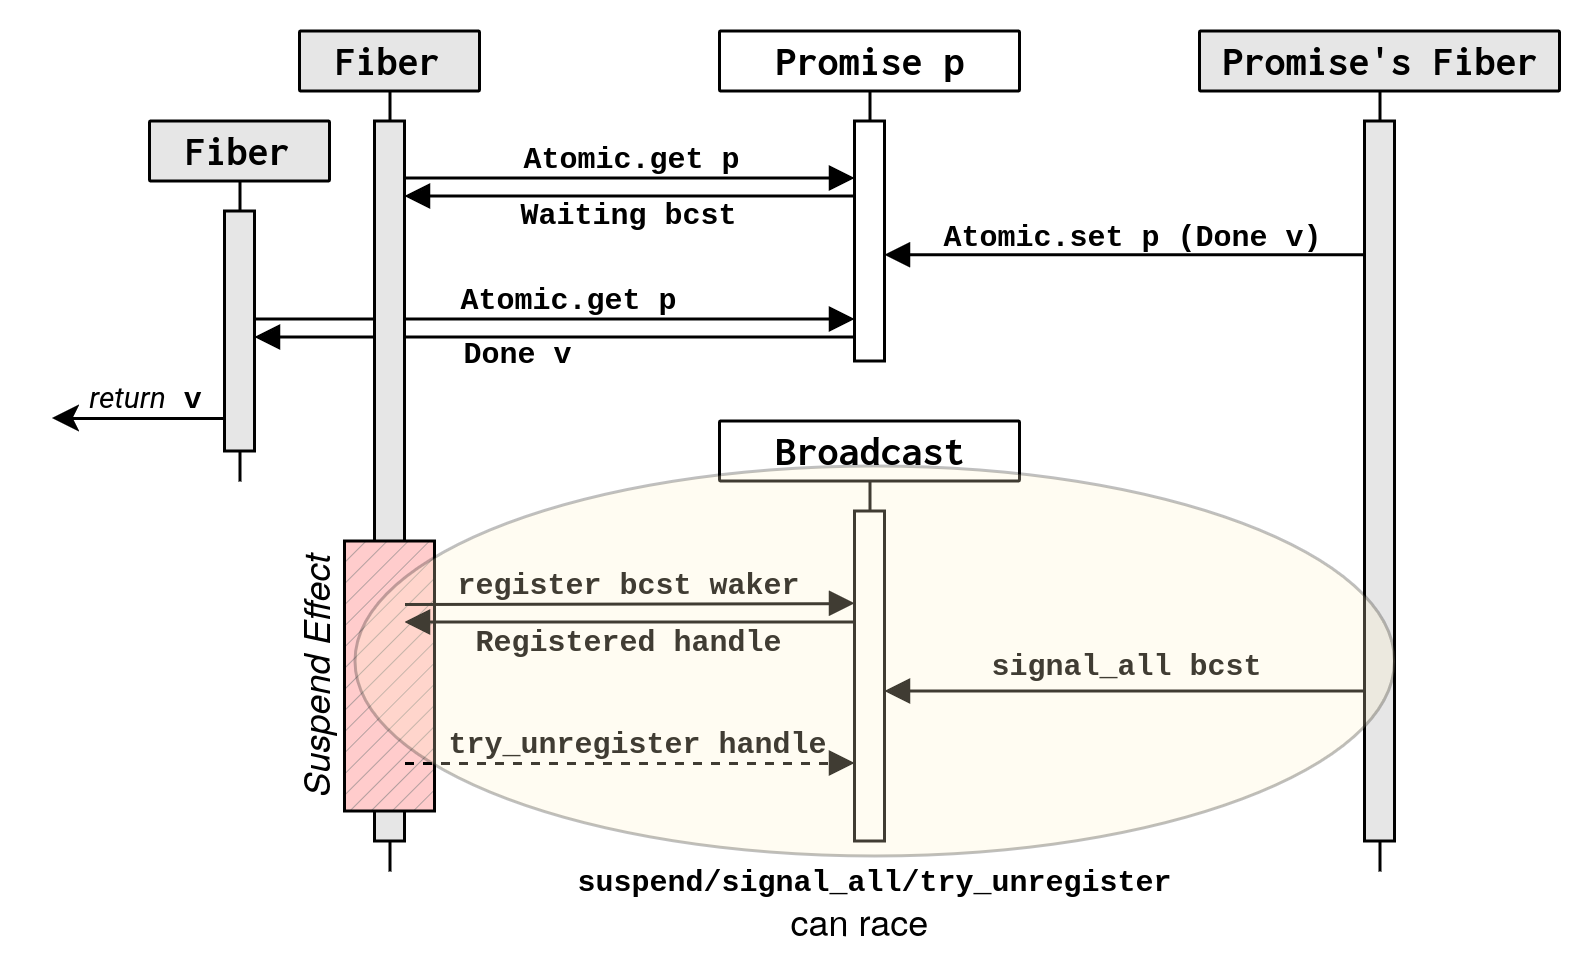
\includegraphics[width=\textwidth]{CQS_Outer_Atomic.png}
  \caption{Usage of CQS with an Outer Atomic Variable}
  \label{fig:cqs-usage}
\end{figure}

Note that because broadcast is a lock-free data structure and fibers can run on different threads, there can be a race between concurrent \emph{register}, \emph{tryCancel}, and \emph{signalAll} operations.
Possible interleavings and the necessity of the \emph{cancel operation} were explained in section~\ref{sec:sched-impl-await}.

\subsection{Implementation and Logical Interface of Broadcast}
\label{sec:broadcast-impl}

% <!-- Some general information how CQS is implemented and the logical state describing the entire queue. -->

CQS is implemented as a queue of \emph{cells} with two pointers pointing to the beginning and end of the active cell range, the \emph{suspend pointer} and the \emph{resume pointer}.
Cells not reachable from either pointer are garbage collected, but their logical state is still tracked.
There is a stack of operations for manipulating these pointers to implement the higher-level functionality, but they are not part of the public API, so we do not focus on them.
Each cell is a container for one callback and the logical state of the queue tracks the logical state of all existing cells.
The possible logical states for a single cell are shown in figure~\ref{fig:cqs-cell-states} and there exist logical operations to change a cell's state.

The number of active cells \(n\) (i.e. the length of the queue) is tracked by the logical resource \(CQSState\; n\).
In normal usage of CQS, the atomic variable of the outer synchronization construct would encode the length of the queue in its value and keep this resource in an associated invariant.
Changing the length of the queue is done using \emph{enqueue} and \emph{dequeue registration} logical operations when opening this invariant.

However, for promises the exact length of the queue is irrelevant because the \emph{signalAll} operation will always set the length to 0.
So in the adapted proof for Eio's broadcast we keep the \(CQSState\; n\) resource in the invariant of the broadcast itself.
As a consequence we also move the \emph{enqueue} and \emph{dequeue registration} out of the public logical API because they are now done internally.

\begin{figure}[ht]
  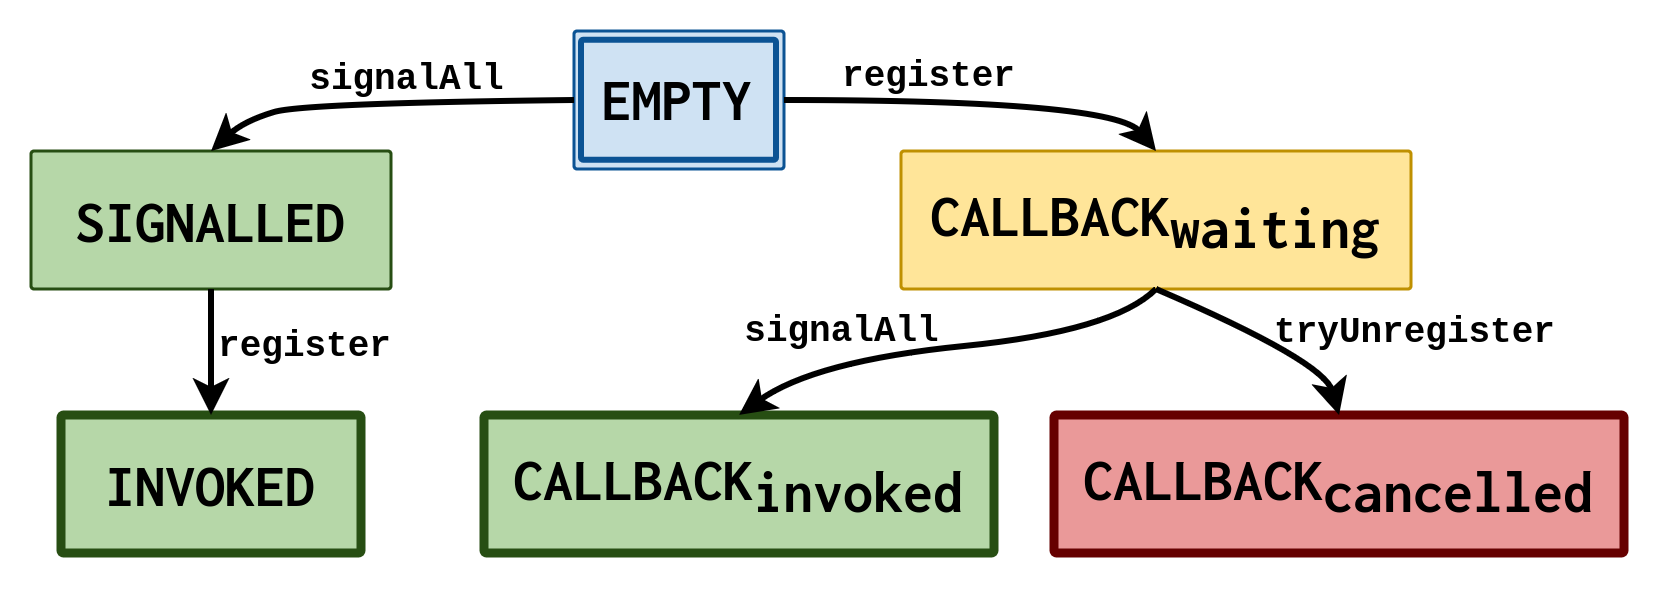
\includegraphics[width=\textwidth]{Cell_States.png}
  \caption{State Transition Diagram for a Single Cell.}
  \label{fig:cqs-cell-states}
\end{figure}

\subsection{Verification of Broadcast}
\label{sec:broadcast-spec}

In the following we describe the specifications we proved for the functions implemented in Eio's \ocamlin{Broadcast} module, and what changes we did to the internal logical state of CQS to carry out the proofs.
For all three operations, the Eio implementation differs from the implementation already verified in the original CQS (e.g. some reordered instructions or a slightly different control flow) and they have different specifications.
However, the specifications of the underlying operations for manipulating cell pointers are modular enough to allow us to prove the new specifications for \ocamlin{Broadcast.create}, \ocamlin{Broadcast.register}, and \ocamlin{Broadcast.try_cancel}.

As for \ocamlin{Broadcast.signal_all}, Eio implements this function by atomically increasing the \emph{resume pointer} by the number \(n\) of registered callbacks and then processing all \(n\) cells between the old and new pointer position.
Because of technical differences between the original CQS implementation of~\cite{koval2023cqs} and the broadcast implementation of Eio we opted to verify a different implementation of \ocamlin{Broadcast.signal_all}, that increments the \emph{resume pointer} \(n\) times in a loop.
We argue this does not change the observable behaviors of the function since we ensure that it can only be called once.

\subsubsection{\ocamlin{Broadcast.create}}
\label{sec:broadcast-spec-create}

Creating a broadcast requires \(inv\_heap\_inv\) which is an Iris proposition which says that we are in a garbage-collected setting.
As a result we get the persistent \(\gsIsBcst{}\; bcst\) resource that shows the value \(bcst\) is a broadcast.
We also obtain the unique resource \gssignal{}, which is held by the enclosing promise and allows calling the \ocamlin{Broadcast.signal_all} function once.

\[
  \inferrule[Spec-BroadcastCreate]
  {inv\_heap\_inv}
  {\ewp{create\; ()}{\bot}{bcst,\; \gsIsBcst{}\; bcst \ast \gssignal{}}}
\]

\subsubsection{\ocamlin{Broadcast.register}}
\label{sec:broadcast-spec-suspend}

% For a \emph{register} operation the \emph{suspend permit} from the original CQS is not needed anymore since we do the \emph{enqueue registration} internally.
A \emph{register} operation takes a callback \(cb\) and the associated resource \(\gsIsCb{}\; cb\) which represents the permission to invoke the callback.
We instantiate \(R\) with \gspdone{} so that the callback transports the knowledge that the promise has been fulfilled.
\(\gsIsCb{}\) is not persistent because the callback must be invoked only once, and it might be accessed from a different thread.

\begin{align*}
  \gsIsCb{}\; cb\; R                            & \triangleq R \wand \ewp{cb\; ()}{\bot}{\top}                                                           \\
  \emph{isBroadcastRegisterResult}\; r\; cb\; R & \triangleq (\ulcorner r = Called \urcorner)                                                            \\
                                                & \quad \vee (\ulcorner r = Registered\; h \urcorner \ast \emph{isBroadcastRegisterHandle}\; h\; cb\; R) \\
  \emph{isBroadcastRegisterHandle}              & : Val \to Val \to iProp \to iProp
\end{align*}


The \ocamlin{Broadcast.register} function will advance the \emph{suspend pointer} to allocate a fresh cell in the \textbf{EMPTY} logical state.
If there is a concurrent call to \ocamlin{Broadcast.signal_all} which changed the cell to the \textbf{RESUMED} logical state before this function can save the callback into the fresh cell, the callback is invoked immediately and the value \(Called\) is returned.
In this case, the state of the cell will be set to \textbf{TAKEN}.
Otherwise, the callback is saved in the cell, which is advanced to the \textbf{CALLBACK(waiting)} logical state, and a \(Registered\; handle\) value is returned along with a \(\textit{isBroadcastRegisterHandle}\) resource as the cancellation permit.

\[
  \inferrule[Spec-BroadcastRegister]
  { \gsIsBcst{}\; bcst \ast \gsIsCb{}\; callback\; R }
  { \ewp{register\; bcst\; callback}{\bot}{r,\; \emph{isBroadcastRegisterResult}\; r\; callback\; R}}
\]

\subsubsection{\ocamlin{Broadcast.try_cancel}}
\label{sec:broadcast-spec-cance}

Given a \(textit{isBroadcastRegisterHandle}\; h\; cb\; R\), \ocamlin{Broadcast.try_cancel} will try to cancel the registration of the callback.

If the callback had already been invoked by a call to \ocamlin{Broadcast.signal_all} (i.e. the logical state is \textbf{CALLBACK(resumed)}) the function returns \ocamlin{false} and no resources are returned to the caller.
Otherwise, the permission to invoke the callback \(\gsIsCb{}\; cb\) is returned, and the cell is advanced to the \textbf{CALLBACK(cancelled)} logical state.

\[
  \inferrule[Spec-BroadcastTryCancel]
  { \emph{isBroadcastRegisterHandle}\; h\; cb\; R }
  { \ewp{try\_cancel\; h}{\bot}{b,\; if\; b\; then\; \gsIsCb{}\; cb\; R\; else\; \top}}
\]

\subsubsection{\ocamlin{Broadcast.signal_all}}
\label{sec:broadcast-spec-signal-all}

To call \ocamlin{Broadcast.signal_all} the unique \(\gssignal{}\) resource is needed.
The \ocamlin{R} resource must be duplicable because it will be used to invoke multiple callbacks, which have \ocamlin{R} as their precondition.
The function does not return any resources because its only effect is making an unknown number of fibers resume execution, which is not something we can easily formalize in Iris.

\[
  \inferrule[Spec-BroadcastSignalAll]
  { \gsIsBcst{}\; bcst \ast \always{}\;R \ast \gssignal{}}
  { \ewp{signalAll\; bcst}{\bot}{\top} }
\]

\subsection{Features Removed from Original CQS}
\label{sec:broadcast-spec-removed-features}

The original CQS supports multiple additional features like a synchronous mode for suspend and resume, and also a smart cancellation mode.
These features enlarge the state space of CQS and complicate the verification but are not used in Eio so when we ported the verification of CQS to our Eio development we removed support for these features.
This reduced the state space of a cell shown in figure~\ref{fig:cqs-cell-states-original} to something more manageable for us when adapting the proofs.

\begin{figure}[ht]
  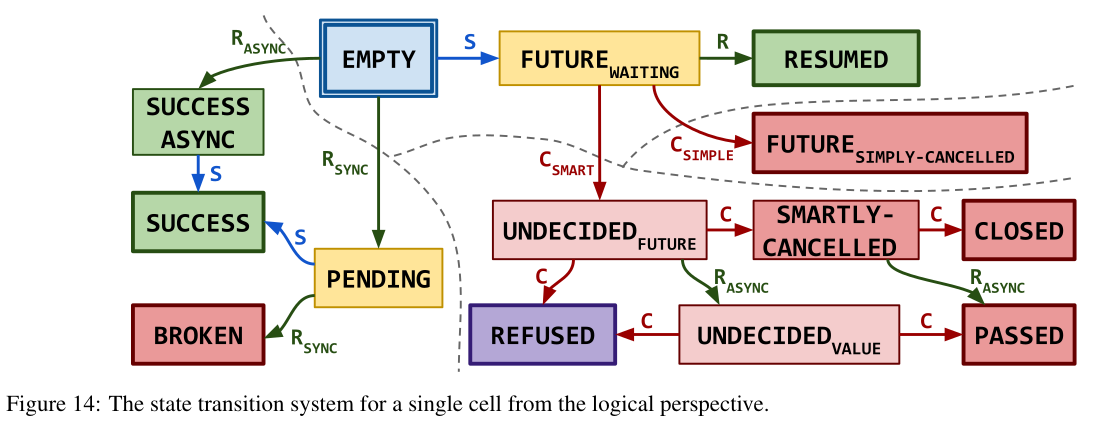
\includegraphics[width=\textwidth]{Cell_States_Original.png}
  \caption{Cell States in the Original CQS from~\cite{koval2023cqs} (page 42).}
  \label{fig:cqs-cell-states-original}
\end{figure}

The part of the verification of the original CQS that we had to customize for Eio was originally 3600 lines of Coq code but -- due to these simplifications -- we could reduce it by approximately 1300 lines of Coq code.
Additionally, there are ~4000 lines of Coq code about lower-level functionality that we did not need to adapt when porting them to our development.
